The \textit{Home Screen} is the entry point to the web application (siehe Figure~\ref{fig:homescreen}).
From here the user can \textit{upload an existing task} (label 1), \textit{create a new task} (label 2), \textit{see a list of saved tasks} (label 3) and \textit{fill out a rubric} (label 4). The labels are further described below.

\begin{itemize}
  \item[\textbf{1:}] The user can upload a \textit{task}, a JSON-File in order to fill out the rubric.
  \item[\textbf{2:}] The user can create an entirely new \textit{task}.
  \item[\textbf{3:}] The user can view a list of \textit{tasks} available for assessment.
  \item[\textbf{4:}] The user can start the \textit{assessment process} and fill out an existing task.
\end{itemize}

\begin{figure}[h]
  \begin{center}
    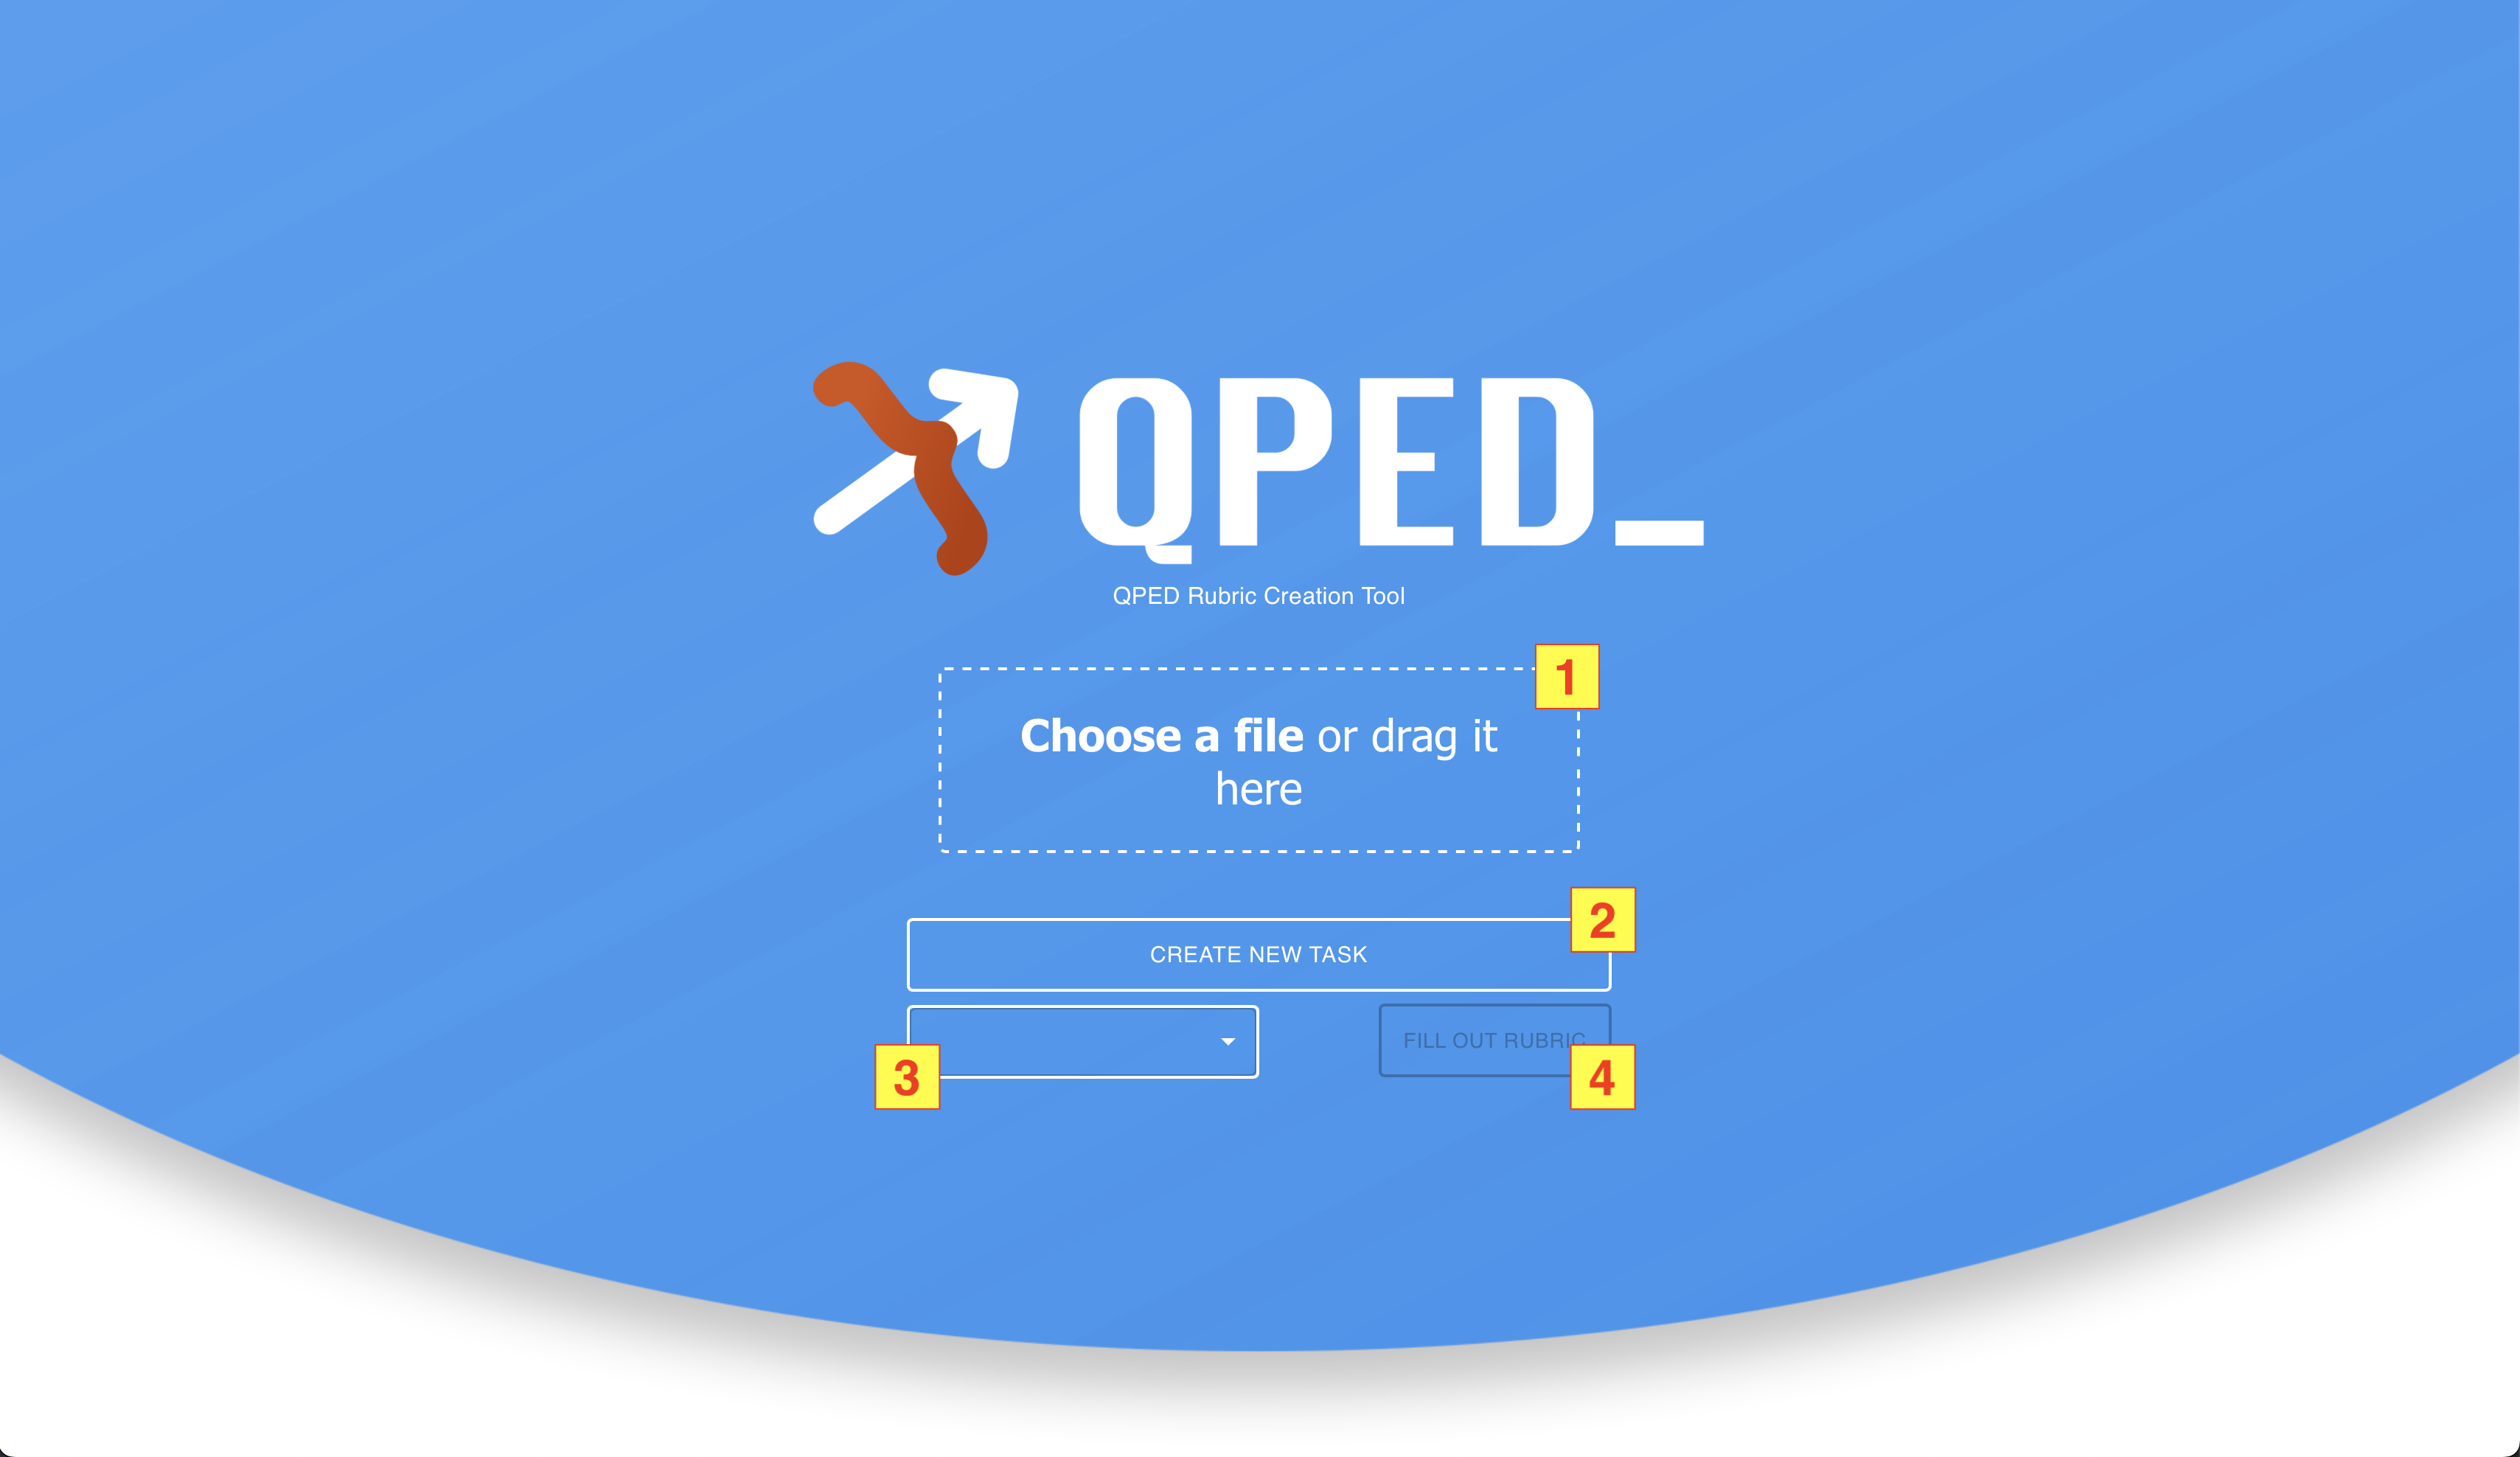
\includegraphics[width=0.9\textwidth]{figures/homescreen}
  \end{center}
  \caption{Screenshot of the \nameref{sec:home}}
  \label{fig:homescreen}
\end{figure}

